\section{Overview of Actario}
\label{sec:overview}

\subsection{Programming in Actario}

Actario is a Coq framework for defining and verifying actor-based
systems. A typical workflow using Actario is as follows.
\begin{enumerate}
\item Describe an actor-based system using types and notations defined in the framework.
\item Specify and verify desired properties of the system.
\item Extract the Erlang version of the system using the code extraction mechanism of Coq.
\end{enumerate}

Actario is currently under development and still does not provide
convenient libraries of predicates, lemmas, tactics and so
forth. Thus, verifying a user-defined actor system may involve a large
amount of work. However, we have formally proved that the underlying
execution model provided in the framework satisfies three important
actor properties: name uniqueness, actor persistence and name
persistence. The fact implies that a system described using Actario is
guaranteed to have these actor properties.

\paragraph{Example: Recursive Factorial System}
Let us use a simple example to illustrate the usage of Actario.
Figure~\ref{coq:fact} is the definition of an actor system that implements the
continuation-passing style factorial function adapted from
\cite{Agha:1986aa}.  Two recursive functions \lstinline|factorial_behv| and
\lstinline|factorial_cont_behv| define the behaviors of factorial actors and
continuation actors respectively.  The function \lstinline|factorial_system| the
system by being applied to a natural number and the name of a customer
actor that is intended to receive the final result.  In this function,
a factorial actor is created and bound to the variable \lstinline|x|, then a pair
of the number and customer is sent to the actor.

\begin{figure}[t]
\begin{lstlisting}[style=small]
CoFixpoint factorial_cont_behv (val : nat)
                               (cust : name) :=
  receive (fun msg =>
    match msg with
     | nat_msg arg => cust ! nat_msg (val * arg);
                      become empty_behv
     | _ => become (factorial_cont_behv val cust)
    end).

CoFixpoint factorial_behv :=
  receive (fun msg =>
    match msg with
     | tuple_msg (nat_msg 0) (name_msg cust) =>
       cust ! nat_msg 1;
       become factorial_behv
     | tuple_msg (nat_msg (S n)) (name_msg cust) =>
       cont <- new (factorial_cont_behv (S n) cust);
       me <- self;
       me ! tuple_msg (nat_msg n) (name_msg cont);
       become factorial_behv
     | _ => become factorial_behv
    end).

Definition factorial_system (n : nat) (cust : name) :=
  init "factorial" (
    x <- new factorial_behv;
    x ! tuple_msg (nat_msg n) (name_msg cust);
    become empty_behv
  ).
\end{lstlisting}
\caption{Recursive Factorial System in Actario}\label{coq:fact}
\end{figure}

%% \begin{figure}[t]
%% \centering
%% 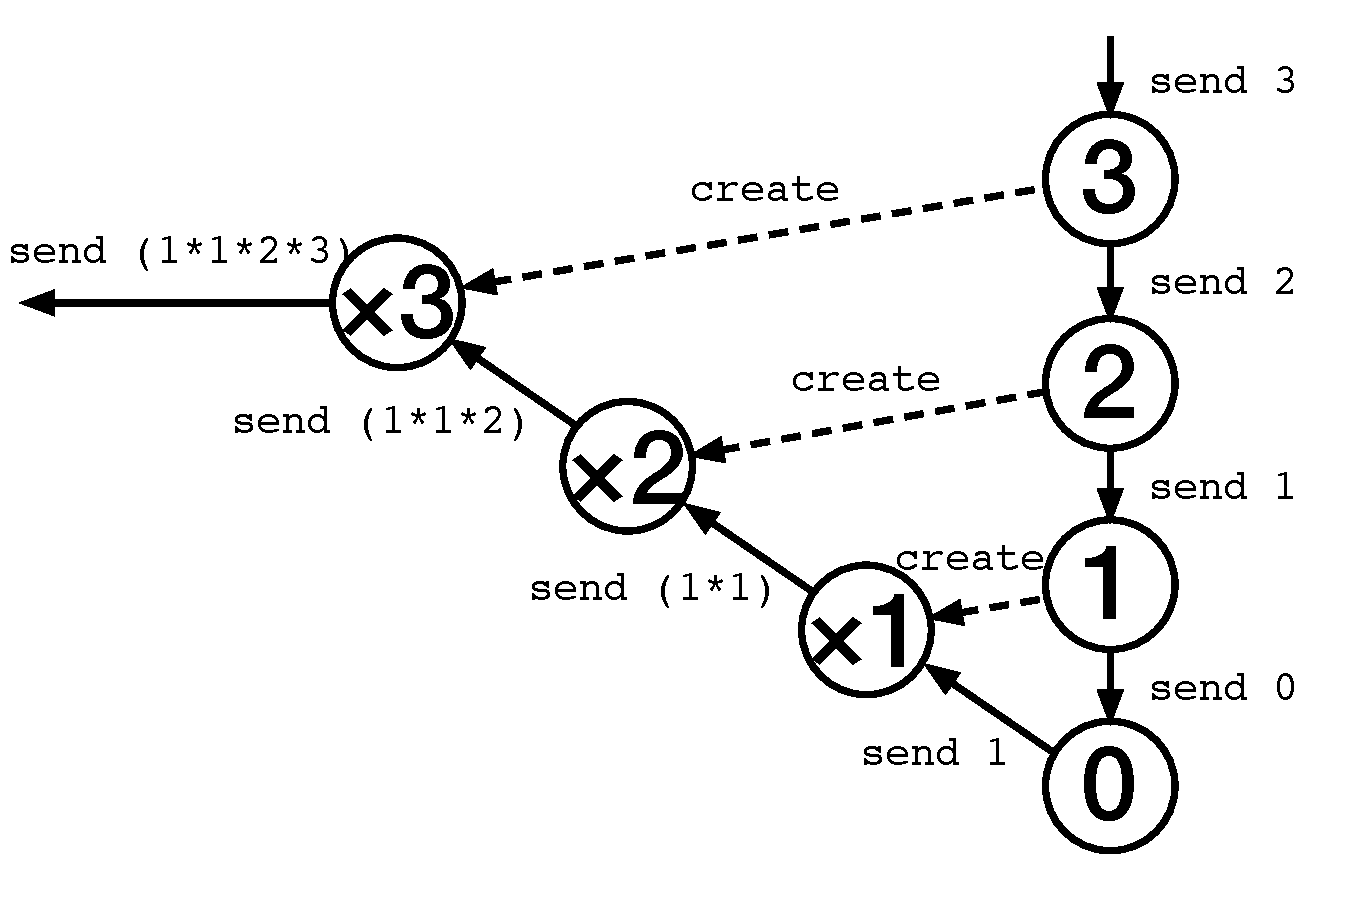
\includegraphics[width=8cm]{./images/fact.pdf}
%% \caption{Recursive Factorial}\label{fig:fact}
%% \end{figure}


\subsection{Types and Notations}

\subsubsection{Messages}
アクター間で取り交わされるメッセージの型 \texttt{message} は図\ref{coq:message}と定義されている。
空のメッセージ、アクターの名前のメッセージ、基本的な型 (自然数、文字列、ブール値) のメッセージ、タプルのメッセージを扱うことができる。

\begin{figure}[tb]
\begin{lstlisting}
Inductive message : Set :=
 | empty_msg : message
 | name_msg : name -> message
 | str_msg : string -> message
 | nat_msg : nat -> message
 | bool_msg : bool -> message
 | tuple_msg : message -> message -> message.
\end{lstlisting}
\caption{Message Type}\label{coq:message}
\end{figure}


\subsubsection{Actions and Behaviors}

\texttt{actions} はアクターが行うアクションの列を表す型である。
アクションの種類は、他のアクターに向けてメッセージを送る\texttt{send}、新しいアクターを作る\texttt{new}、自分自身の名前を得る\texttt{self}、次のメッセージに対する振る舞いを決める\texttt{become}があり、これらが \texttt{actions} の値コンストラクタとなっている。
behavior is defined as a function from message to actions.

\begin{figure}[tb]
\begin{lstlisting}
CoInductive actions : Type :=
 | new : behavior -> (name -> actions) -> actions
 | send : name -> message -> actions -> actions
 | self : (name -> actions) -> actions
 | become : behavior -> actions
with behavior : Type :=
 | receive : (message -> actions) -> behavior.
\end{lstlisting}
\caption{Types for Actions and Behaviors}\label{coq:actions}
\end{figure}

\texttt{actions} および \texttt{behavior} は Actario では図\ref{coq:actions} のように定義されている。
\texttt{actions} のそれぞれのコンストラクタを説明する。

\begin{list}{}{%
%    \setlength{\labelwidth}{0pt}
%    \setlength{\labelsep}{0pt}
    \setlength{\leftmargin}{1.5em}
    \setlength{\itemindent}{-1.5em}
}
\item \lstinline|new : behavior -> (name -> actions) -> actions|\\
  新しいアクターを生成するアクションである。
  引数として与えられたある behavior を initial behavior として新しいアクターを生成し、その名前をアクションの継続に渡す。
\item \lstinline|send : name -> message -> actions -> actions|\\
  指定した名前のアクターにメッセージを送るアクションである。
  第一引数に指定した名前のアクターに、第二引数で指定したメッセージを送り、第三引数で指定したその後のアクションを実行する、という意味である。
\item \lstinline|self : (name -> actions) -> actions| \\
  自分自身の名前を得るアクションである。
  自分の名前を第一引数で与えられた継続に渡し、残りのアクションを得る。
\item \lstinline|become : behavior -> actions| \\
  次のメッセージに対して指定した振る舞いで処理する。
  また、次のメッセージの待ち状態になることも表し、これ以降アクションは取れないようになっている。
\end{list}

actions と behavior は co-inductive types として定義される。
これは become で現在の behavior を指定したり、ある他の behavior と相互再帰するようなことがあるからである。
Coq ではこのような、コンストラクタの深さが小さくならない再帰は通常の inductive definition では書けなくなっている。

\subsubsection{Notations}

また、アクターモデルを採用しているプログラミング言語に近づけるように図\ref{coq:notation}のような notation をつけている。
\lstinline|n <- new behv; cont| は \lstinline|new behv (fun n => cont)| に変換され、
\lstinline|n ! msg; cont| は \lstinline|send n msg cont| に変換され、
\lstinline|me <- self; cont| は \lstinline|self (fun me => cont)| に変換される。

\begin{figure}[tb]
\begin{lstlisting}
Notation ``n '<-' 'new' behv ; cont'' :=
    (new behv (fun n => cont))
    (at level 0, cont at level 10).
Notation ``n '!' m ';' a'' :=
    (send n m a) (at level 0, a at level 10).
Notation ``me '<-' 'self' ';' cont'' :=
    (self (fun me => cont))
    (at level 0, cont at level 10).
\end{lstlisting}
\caption{Notations for Actions}\label{coq:notation}
\end{figure}
